
%packages
\usepackage{natbib}
\usepackage{amsmath}
\usepackage{amsthm}
\usepackage{mathtools}
\usepackage{mdframed}
\usepackage{subfigure}
\usepackage{booktabs}
% \usepackage{hyperref}
\usepackage{subfigure}
\usepackage{siunitx} % Provides the \SI{}{} and \si{} command for typesetting SI units
\usepackage{graphicx} % Required for the inclusion of images
% \usepackage{natbib} % Required to change bibliography style to APA
\usepackage{datetime}
\usepackage{lscape}
\usepackage{algorithm}
\usepackage{algorithmic}
\usepackage{xspace}
\usepackage[english]{babel} % English language/hyphenation
\usepackage{proof}
\usepackage{booktabs} % Top and bottom rules for tables
\usepackage[colorlinks, allcolors = blue,]{hyperref}
\usepackage{accents}
\usepackage{amsfonts}
\usepackage{stmaryrd}
\usepackage{amsmath,amsthm,amssymb,latexsym} 
\usepackage{microtype}
\usepackage{graphicx}
\usepackage{subfigure}
\usepackage{booktabs} % for professional tables
\usepackage{hyperref}
\usepackage{icml2019}
\usepackage{lipsum}

\usepackage{authblk}


%new commands
\newcommand{\theHalgorithm}{\arabic{algorithm}}
\newtheorem{definition}{Definition}
\usepackage{cancel}
\usepackage[normalem]{ulem}
\newcommand{\dataobs}{\textbf{x}}
\newcommand{\adj}[2]{\textbf{adj}(#1,#2)}
\newcommand{\candidateset}{\mathcal{R}_{\textup{post}}}
\newcommand{\bprior}{\boldsymbol{\beta}_{\textup{prior}}}
\newcommand{\bysinfer}{\mathsf{Infer}}
\newcommand{\betad}{\mathsf{Beta}}
\newcommand{\betaf}{\textup{B}}
\newcommand{\mbetaf}{\boldsymbol{\textup{B}}}
\newcommand{\vtheta}{\boldsymbol{\theta}}
\newcommand{\valpha}{\boldsymbol{\alpha}}
\newcommand{\vbeta}{\boldsymbol{\beta}}
\newcommand{\lapmech}{\mathsf{LSDim}}
\newcommand{\ilapmech}{\mathsf{LSHist}}
\newcommand{\binomial}[2]{\mathsf{Bin}(#1, #2)}
\newcommand{\multinomial}[2]{\mathsf{Mult}(#1, #2)}
\newcommand{\expmech}{\mathsf{EHD}}
\newcommand{\hexpmech}{\mathsf{EHDS}}
\newcommand{\lexpmech}{\mathsf{EHDL}}
\newcommand{\hexpmechd}{\mathsf{expMech}^{D}_{\hellinger}}
\newcommand{\privinfer}{\mathsf{PrivInfer}}
\newcommand{\hlg}{\mathsf{H}}
\newcommand{\dirichlet}[1]{\mathsf{Dir}(#1)}
\newcommand{\alphas}{\boldsymbol{\alpha}}
\newcommand{\xis}{\boldsymbol{\xi}}
\newcommand{\iverson}[1]{[#1]}
\newcommand{\datauni}{\mathcal{X}}
\newcommand{\hellinger}{\mathcal{H}}
\newcommand{\ux}[1]{u(\textbf{x}, {#1})}
\newcommand{\uxadj}[1]{u(\textbf{x}', {#1})}
\newcommand{\cardinality}[2]{\mathcal{C}^{#1}_{#2}}
\newcommand{\range}{\mathcal{O}}
\newcommand{\nomalizer}[1]{\sum\limits_{r'\in \mathcal{R}_{\textup{post}}} \exp \big(\frac{-\epsilon\cdot \mathcal{H} (\mathsf{BI}(#1),r')}{4 \cdot S(#1)}\big)}

\newcommand{\unomalizer}[1]{\sum\limits_{r'\in \mathcal{R}_{\textup{post}}} \exp \big(\frac{-\epsilon\cdot u(#1, r')}{4 \cdot S(#1)}\big)}


\newcommand{\hexpmechPr}[2]{\underset{z \thicksim \hexpmech(#1)}{\Pr}\left[ #2 \right]}
\newcommand{\lapmechPr}[2]{\underset{z \thicksim \lapmech(#1)}{\Pr}\left[ #2 \right]}

\newcommand{\ilapmechPr}[2]{\underset{
{z \thicksim \ilapmech(#1)}
}{\Pr}\left[ #2 \right]}

\newtheorem{thm}{Theorem}[section]

\newtheorem{lem}{Lemma}[section]

\newtheorem{assert}{Assertion}[lem]
\newcommand{\lap}[2]{\mathsf{Lap}(#1, #2)}
\newcommand{\todo}[1]{{\footnotesize \color{red}\textbf{[[ #1 ]]}}}

\title{\textbf{Notes of DP - Bayesian Inference}\\}
% \author{Jiawen \textsc{Liu}}
\date{\vspace{-10ex}}

\begin{document}
\maketitle

\section{Bayesian Inference Based on Dirichlet-Bernoulli Distribution}
\label{sec_bayesInfer}
In the Bayesian inference, first there is a prior distribution $\pi(\xis)$ to present our belief about parameter $\xis$. Then, we get some observed data $x$ sizing $n$, and produce a posterior distribution $Pr(\xis | x)$. The Bayesian inference is based on the Bayes' rule to calculate the posterior distribution:
\begin{equation*}
Pr(\xis | x) = \frac{Pr(x | \xis) \pi(\xis)}{Pr(x)}
\end{equation*}
It is denoted as $\bysinfer(x,\pi(\xis))$ taking an observed data set $x \in \mathcal{X}^n$ and a prior distribution $\pi(\xis)$ as input, outputting a posterior distribution of the parameter $\alphas$. For conciseness, when prior is given, we use $\bysinfer(x)$. $n$ is the size of the observed data size.

In our inference algorithm, we take a Dirichlet distribution as prior belief for the parameters, $\dirichlet(\alphas)$, where $\pi(\xis) = \dirichlet(\xis | \alphas) = \frac{\prod_{i = 1}^{m}\xi_i^{\alpha_i}}{B(\alphas)}$, and the Bernoulli distribution as the statistic model for $Pr(x | \alphas)$. $m$ is the order of the Dirichlet distribution.

We give a inference process based on a concrete example, where we throw an irregular $m$ sides dice. We want to infer the probability of getting each side $\xis$. We get a observed data set $\{s_{k_1}, s_{k_2}, \cdots, s_{k_n}\}$ by throwing the dice $n$ times, where $k_i \in \{1,2,\cdots, m\}$ denotes the side we get when we throw the dice the $i^{th}$ time. The posterior distribution is still a Dirichlet distribution with parameters $(\alpha_1 + n_1, \alpha_2 + n_2, \cdots, \alpha_m + n_m)$, where $n_i$ is the appearance time of the side $i$ in total.

In the case that $m = 2$, it is reduced to a Beta distribution $\betad(\alpha, \beta)$. The $m$ side dice change into a irregular coin with side $A$ and side $B$. The posterior is computed as $(\alpha + n_1, \beta + n_0)$, where $n_1$ is the appearance time of side $A$ in the observed data set and $n_0$ is the appearance time of the other side.



\section{Algorithm Setting up}
\label{sec_setup}
For now, we already have a prior distribution $\pi(\xis)$, an observed data set $x$.

\subsection{Exponential Mechanism with Global Sensitivity}
\label{subsec_emgs}

% \subsubsection{Mechanism Set up}

In exponential mechanism, candidate set $\mathcal{R}$ can be obtained by enumerating $y \in \mathcal{X}^n$, i.e.
\begin{equation*}
\mathcal{R} = \{\bysinfer(y)\ |\ y \in \mathcal{X}^n\}.
\end{equation*}

Hellinger distance $\hlg$ is used here to score these candidates. The utility function:
\begin{equation}
\label{equ_utility}
u(x,r) = -\hlg(\bysinfer(x), r); r \in \mathcal{R}.
\end{equation}

Exponential mechanism with global sensitivity selects and outputs a candidate $r \in \mathcal{R}$ with probability proportional to $exp(\frac{\epsilon u(x,r)}{2 \Delta_{g}u})$:
\begin{equation*}
P[r] = \frac
{exp(\frac{\epsilon u(x,r)}{2 \Delta_{g}u})}
{\Sigma_{r' \in \mathcal{R}}\ exp(\frac{\epsilon u(x,r')}{2 \Delta_{g}u})},
\end{equation*}
where global sensitivity is calculated by:
\begin{equation*}
\Delta_{g}u = 
\max_{\{|x',y'| \leq 1;x',y'\in \mathcal{X}^n\}}\max_{\{r\in \mathcal{R}\}}
|\hlg(\bysinfer(x'), r) - \hlg(\bysinfer(y'), r)|
\end{equation*}

The basic exponential mechanism is $\epsilon -$differential privacy\cite{dwork2014algorithmic}.

% We use probability proportional to $exp(\frac{\epsilon u(x,r)}{\Delta_{g}u})$ rather than $exp(\frac{\epsilon u(x,r)}{2 \Delta_{g}u})$. Since $\hlg$ is monotonic, i.e. our utility function is monotonic. 

% \subsubsection{Security Analysis}
% It can be proved that exponential mechanism with global sensitivity is $\epsilon$-differentially private. We denote the $\bysinfer$ with privacy mechanism as $\privinfer$. For adjacent data set $||x,y||_1 = 1$:
% \begin{equation*}
% \begin{split}
% \frac{P[\privinfer(x,u,R) = r]}{P[\privinfer(y,u,R) = r]}
% & =\frac
% {\frac
% {exp(\frac{\epsilon u(x,r)}{2 \Delta_{g}u})}
% {\Sigma_{r' \in R}\ exp(\frac{\epsilon u(x,r')}{2 \Delta_{g}u})}}
% {\frac
% {exp(\frac{\epsilon u(y,r)}{2 \Delta_{g}u})}
% {\Sigma_{r' \in R}\ exp(\frac{\epsilon u(y,r')}{2 \Delta_{g}u})}} \\
% & = \left(\frac
% {exp(\frac{\epsilon u(x,r)}{2 \Delta_{g}u})}
% {exp(\frac{\epsilon u(y,r)}{2 \Delta_{g}u})}
% \right)
% \cdot
% \left(\frac
% {\sum\limits_{r' \in R}\ exp(\frac{\epsilon u(y,r')}{2 \Delta_{g}u})}
% {\sum\limits_{r' \in R}\ exp(\frac{\epsilon u(x,r')}{2 \Delta_{g}u})}
% \right)\\
% & = exp\left(\frac
% {\epsilon (u(x,r) - u(y,r))}
% {2 \Delta_{g}u}
% \right)
% \cdot
% \left(\frac
% {\sum\limits_{r' \in R}\ exp(\frac{\epsilon u(y,r')}{2 \Delta_{g}u})}
% {\sum\limits_{r' \in R}\ exp(\frac{\epsilon u(x,r')}{2 \Delta_{g}u})}
% \right)\\
% & \leq
% exp(\frac{\epsilon}{2}) \cdot exp(\frac{\epsilon}{2}) \cdot
% \left(\frac
% {\sum\limits_{r' \in R}\ exp(\frac{\epsilon u(x,r')}{2 \Delta_{g}u})}
% {\sum\limits_{r' \in R}\ exp(\frac{\epsilon u(x,r')}{2 \Delta_{g}u})}
% \right)\\
% & = exp(\epsilon).
% \end{split}
% \end{equation*}

% Then, $\frac{P[\privinfer(x,u,R) = r]}{P[\privinfer(y,u,R) = r]} \geq exp(-\epsilon)$ can be obtained by symmetry.


\subsection{Exponential Mechanism with Local Sensitivity}
\label{subsec_emls}
% \subsubsection{Mechanism Set up}
Exponential mechanism with local sensitivity share the same candidate set and utility function as it with global sensitivity. This outputs a candidate $r \in \mathcal{R}$ with probability proportional to $exp(\frac{\epsilon u(x,r)}{2 \Delta_{l}u})$:
\begin{equation*}
P[r] = \frac
{exp(\frac{\epsilon u(x,r)}{2 \Delta_{l}u})}
{\Sigma_{r' \in \mathcal{R}}\ exp(\frac{\epsilon u(x,r')}{2 \Delta_{l}u})},
\end{equation*}

where local sensitivity is calculated by:

\begin{equation*}
\Delta_{l}u(x) = 
\max_{\{|x,y'| \leq 1;y'\in \mathcal{X}^n\}}\max_{\{r\in \mathcal{R}\}}.
\hlg(\bysinfer(x), r) - \hlg(\bysinfer(y'), r)|
\end{equation*}

The exponential mechanism with local sensitivity is non differential privacy\cite{dwork2014algorithmic}.


\subsection{Exponential Mechanism with Smooth Sensitivity}
\label{sec_smoo}

\subsubsection{Algorithm Setting up}
We define a new mechanism $\hexpmech(x)$
which is similar to the exponential mechanism where we use
$\mathcal{R}$ as the set $\betaset$ of beta distributions with integer parameters
summing up to $n+2$, as scoring function we use the Hellinger distance
from $\bysinfer(x)$, i.e. $\hlg(\bysinfer(x),-)$, and we 
calibrate the noise to the smooth sensitivity~\cite{nissim2007smooth}. The
only difference is in the sensitivity part, since now we use the
smooth sensitivity.

\begin{definition} The mechanism $\hexpmech(x)$ outputs a candidate $r \in \betaset$ with probability
\begin{equation*}
\underset{z \thicksim \hexpmech(x)}{Pr}[z=r] = \frac
{exp(\frac{-\epsilon\hlg(\bysinfer(x),r)}{2 S_\beta(x)})}
{\Sigma_{r' \in R}\ exp(\frac{-\epsilon \hlg(\bysinfer(x),r')}{2 S_\beta(x)})},
\end{equation*}
where $s_\beta(x)$ is the smooth sensitivity of $\hlg(\bysinfer(x),-)$, calculated by:
\begin{equation*}
S_{\beta}(x) = \max(\Delta_{l}\hlg(\bysinfer(x),-), \max_{y \neq x; y \in D^{n}}(\Delta_{l}\hlg(\bysinfer(x),-)\cdot e^{-\beta d(x,y)})),
\end{equation*}
where $d$ is the Hamming distance between two datasets, and $\beta =
\beta(\epsilon, \delta)$ is a function of $\epsilon$ and $\delta$. 
\end{definition}


In what follows, we will use a correspondence between the probability
 $\underset{z \thicksim \hexpmech(x)}{Pr}[z = r]$ of every
 $r\in\betaset$ and the probability 
 $\underset{z \thicksim \hexpmech(x)}{Pr}[\hlg(\bysinfer(x),z) =
 \hlg(\bysinfer(x),r)]$ for the utility score for $r$. In particular, for every
 $r\in\betaset$ we have:
$$
\underset{z \thicksim \hexpmech(x)}{Pr}[z = r]=
\frac{1}{2}\Big (\underset{z \thicksim \hexpmech(x)}{Pr}[\hlg(\bysinfer(x),z) =
 \hlg(\bysinfer(x),r)]\Big )
$$
To see this, it is enough to notice that: $\underset{z \thicksim \hexpmech(x)}{Pr}[z = r]$ is proportional too $\hlg(\bysinfer(x),r)$, i.e., $u(x,z)$. We can derive, if $u(r,x) = u(r',x)$ then $\underset{z \thicksim \hexpmech(x)}{Pr}[z = r] = \underset{z \thicksim \hexpmech(x)}{Pr}[z = r']$. We assume the number of candidates $z \in \mathcal{R}$ that satisfy $u(z,x) = u(r,x)$ is $|r|$, we have  $\underset{z \thicksim \hexpmech(x)}{Pr}[u(z,x) = u(r,x)] = |r| \underset{z \thicksim \hexpmech(x)}{Pr}[z = r]$. Because Hellinger distance  $\hlg(\bysinfer(x),z)$ is axial symmetry, where the $\bysinfer(x)$ is the symmetry axis. It can be infer that $|z| = 2$ for any candidates, apart from the true output, i.e., $\underset{z \thicksim \hexpmech(x)}{Pr}[u(z,x) = u(r,x)] = 2 \underset{z \thicksim \hexpmech(x)}{Pr}[z = r]$. This parameter can be eliminate in both sides in proof.

In our private Bayesian inference mechanism, we set the $\beta$ as $\ln(1 - \frac{\epsilon}{2 \ln (\frac{\delta}{2 (n + 1)})})$. 


\subsubsection{Sliding Property of Exponential Mechanism}
\begin{lem}
Consider the exponential mechanism  $\sexpmech(x,u,\mathcal{R})$
calibrated on the smooth sensitivity. Let $\lambda = f(\epsilon,
\delta)$, $\epsilon\geq 0$ and $|\delta| < 1$. Then, the following \emph{sliding property} holds:
\begin{equation*}
\underset{r \thicksim \hexpmech(x)}{Pr}[u(r,x) = \hat{s}]
\leq
e^{\frac{\epsilon}{2}} \underset{r \thicksim \hexpmech(x)}{Pr}[u(r,x) = (\Delta + \hat{s})] + \frac{\delta}{2},
\end{equation*}

\end{lem}

\begin{proof}

We denote the normalizer of the probability mass in $\hexpmech(x)$: $\sum_{r' \in \mathcal{R}}exp(\frac{\epsilon u(r',x)}{2 S(x)})$ as $NL(x)$:
\begin{equation*}
\begin{split}
LHS 
  = \underset{r \thicksim \hexpmech(x)}{Pr}[u(r,x) = \hat{s}]
& = \frac{exp(\frac{\epsilon \hat{s}}{2 S(x)})}{NL(x)}\\
& = \frac{exp(\frac{\epsilon (\hat{s} + \Delta - \Delta)}{2 S(x)})}{NL(x)}\\
& = \frac{exp(\frac{\epsilon (\hat{s} + \Delta)}{2 S(x)} + \frac{- \epsilon \Delta}{2 S(x)})}{NL(x)}\\
& = \frac{exp(\frac{\epsilon (\hat{s} + \Delta)}{2 S(x)})}{NL(x)} \cdot e^{\frac{- \epsilon \Delta}{2 S(x)})}.\\
\end{split}
\end{equation*}

By bounding the $\Delta \geq -S(x)$, we can get:

\begin{equation*}
\begin{split}
\frac{exp(\frac{\epsilon (\hat{s} + \Delta)}{2 S(x)})}{NL(x)} \cdot e^{\frac{- \epsilon \Delta}{2 S(x)}}
& \leq \frac{exp(\frac{\epsilon (\hat{s} + \Delta)}{2 S(x)})}{NL(x)} \cdot e^{\frac{\epsilon}{2}}\\
&  =  e^{\frac{\epsilon}{2}} \underset{z \thicksim \hexpmech(x)}{Pr}[u(r,x) = (\Delta + \hat{s})] \leq RHS\\
\end{split}
\end{equation*}

\end{proof}

\subsubsection{Dilation Property of Exponential Mechanism}
\begin{lem}
for any exponential mechanism $\hexpmech(x)$, $\lambda < |\beta|$, $\epsilon$, $|\delta| < 1$ and $\beta \leq \ln(1 - \frac{\epsilon}{2 \ln (\frac{\delta}{2 (n + 1)})})$, the dilation property holds:

\begin{equation*}
\underset{r \thicksim \hexpmech(x)}{Pr}[u(r,x) = z]
\leq
e^{\frac{\epsilon}{2}} \underset{r \thicksim \hexpmech(x)}{Pr}[u(r,x) = e^{\lambda} z] + \frac{\delta}{2},
\end{equation*}
where the sensitivity in mechanism is still smooth sensitivity as above.
\end{lem}

\begin{proof}

The sensitivity is always greater than 0, and our utility function $-\hlg(\bysinfer(x),r)$ is smaller than zero, i.e., $u(r,x) \leq 0$, we need to consider two cases where $\lambda < 0$, and $\lambda > 0$:

We set the $h(z) = Pr[u(\hexpmech(x)) = z] = 2\frac{exp(\frac{\epsilon z}{2 S(x)})}{NL(x)}$.

We first consider $\lambda < 0$. In this case, $1 < e ^ {\lambda}$, so the ratio $\frac{h(z)}{h(e^{\lambda}z)} = \frac{exp(\frac{\epsilon z}{2 S(x)})}{exp(\frac{\epsilon (z \cdot e^{\lambda})}{2 S(x)})}$ is at most $\frac{\epsilon}{2}$.

Next, we proof the dilation property for $\lambda > 0$, The ratio of $\frac{h(z)}{h(e^{\lambda}z)}$ is $\exp(\frac{\epsilon}{2} \cdot \frac{u(\hexpmech(x)) (1 - e^{\lambda})}{S(x)})$. Consider the event $G = \{ \hexpmech(x) : u(\hexpmech(x)) \leq \frac{S(x)}{(1 - e^{\lambda})}\}$. Under this event, the log-ratio above is at most $\frac{\epsilon}{2}$. The probability of $G$ under density $h(z)$ is $1 - \frac{\delta}{2}$. Thus, the probability of a given event $z$ is at most $Pr[z \cap G] + Pr[\overline{G}] \leq e^{\frac{\epsilon}{2}} Pr[e^{\lambda}z \cap G] + \frac{\delta}{2} \leq e^{\frac{\epsilon}{2}} Pr[e^{\lambda}z] + \frac{\delta}{2}$.\\


\textbf{Detail proof:}
\begin{itemize}

	\item $\lambda < 0$

		The left hand side will always be smaller than 0 and the right hand side greater than 0. This will always holds, i.e.
		\begin{equation*}
		\end{equation*}
	\item $\lambda > 0$


Because $\hat{s} = u(r)$ where $r \thicksim \hexpmech(x)$, we can substitute $\hat{s}$ with $u(\hexpmech(x))$. Then, what we need to proof under the case $\lambda > 0$ is:
\begin{equation*}
u(\hexpmech(x)) \leq \frac{S(x)}{(1 - e ^ {\lambda})}
\end{equation*}
By applying the accuracy property of exponential mechanism, we bound the probability that the equation holds with probability:
\begin{equation*}
\begin{split}
Pr[u(\hexpmech(x)) \leq \frac{S(x)}{(1 - e ^ {\lambda})}] 
& \leq \frac{|\mathcal{R}|exp(\frac{\epsilon S(x)}{(1 - e ^ {\lambda})}/2 S(x))}{|\mathcal{R}_{OPT}| exp(\epsilon OPT_{u(x)}/2 S(x))}\\
\end{split}
\end{equation*}

In our Bayesian Inference mechanism, the size of the candidate set $\mathcal{R}$ is equal to the size of observed data set plus 1, i.e., $n + 1$, and $OPT_{u(x)} = 0$, then we have:
\begin{equation*}
\begin{split}
Pr[u(\hexpmech(x)) \leq \frac{S(x)}{(1 - e ^ {\lambda})}] 
& = (n + 1)exp(\frac{\epsilon S(x)}{(1 - e ^ {\lambda})}/2 S(x))\\
& = (n + 1)exp(\frac{\epsilon}{2 (1 - e ^ {\lambda})})\\
\end{split}
\end{equation*}

When we set $\lambda \leq \ln(1 - \frac{\epsilon}{2 \ln (\frac{\delta}{2 (n + 1)})})$, it is easily to derive that $Pr[u(\hexpmech(x)) \leq \frac{S(x)}{(1 - e ^ {\lambda})}] \leq \frac{\delta}{2}$.

\end{itemize}

\end{proof}

\subsubsection{Privacy Analysis}
\begin{lem}
\label{lem_hexpmech_privacy}
$\hexpmech$ is $(\epsilon, \delta)$-differential privacy.
\end{lem}

\begin{proof}
of Lemma \ref{lem_hexpmech_privacy}: For all neighboring $x, y \in D^n$ and all sets $\mathcal{S}$, we need to show that:
\begin{equation*}
\underset{z \thicksim \hexpmech(x)}{Pr}[ z \in \mathcal{S}] \leq e^{\epsilon} \underset{z \thicksim \hexpmech(y)}{Pr}[z \in \mathcal{S}] + \delta. 
\end{equation*}
Given that $2\Big( \underset{z \thicksim \hexpmech(x)}{Pr}[ z \in \mathcal{S}]\Big) = \underset{z \thicksim \hexpmech(x)}{Pr}[ u(x,z) \in \mathcal{U}]$, let $\mathcal{U}_1 = \frac{u(y,z) - u(x,z)}{S(x)}$, $\mathcal{U}_2 = \mathcal{U} + \mathcal{U}_1$ and $\mathcal{U}_3 = \mathcal{U}_2 \cdot \frac{S(x)}{S(y)} \cdot \ln(\frac{NL(x)}{NL(y)})$. Then,

\begin{equation*}
\begin{split}
2\Big( \underset{z \thicksim \hexpmech(x)}{Pr}[ z \in \mathcal{S}]\Big)
& = \underset{z \thicksim \hexpmech(x)}{Pr}[ u(x,z) \in \mathcal{U}]\\
& \leq e^{\epsilon / 2} \cdot \underset{z \thicksim \hexpmech(x)}{Pr}[ u(x,z) \in \mathcal{U}_2]\\
& \leq e^{\epsilon} \cdot \underset{z \thicksim \hexpmech(x)}{Pr}[ u(x,z) \in \mathcal{U}_3] + e^{\epsilon/2} \cdot \frac{\delta'}{2}\\
& = e^{\epsilon} \cdot \underset{z \thicksim \hexpmech(y)}{Pr}[ u(y,z) \in \mathcal{U}] + \delta = 2\Big( e^{\epsilon} \cdot \underset{z \thicksim \hexpmech(x)}{Pr}[ z \in \mathcal{S}] \Big) + \delta\\
\end{split}
\end{equation*}

The first inequality holds by the sliding property, since the $\mathcal{U}_1 \geq -S(x)$. The second inequality holds by the dilation property, since $\frac{S(x)}{S(y)} \cdot \ln(\frac{NL(x)}{NL(y)}) \leq 1 - \frac{\epsilon}{2 \ln (\frac{\delta}{2 (n + 1)})}$.

\end{proof}

\section{Accuracy Analysis}
\subsection{Laplace Mechanism}
Fixing a data set $x$, we already had the accuracy bound based on the $l_1$ norm as:
\begin{equation*}
Pr[||Lap(\bysinfer(x)) - \bysinfer(x)||_1 \geq |x| \ln (\frac{m}{\gamma}) \frac{2}{\epsilon}] \leq \gamma,
\end{equation*}
where $m$ is the order of the Dirichlet distribution. Then we have the accuracy bound based on $\hlg$ distance.
\begin{equation*}
\begin{split}
Pr[||Lap(\bysinfer(x)) - \bysinfer(x)||_1 \geq m \ln (\frac{m}{\gamma}) \frac{2}{\epsilon}] & \leq Pr[m ||Lap(\bysinfer(x)) - \bysinfer(x)||_{\infty} \geq m \ln (\frac{m}{\gamma}) \frac{2}{\epsilon}]\\
& = Pr[||Lap(\bysinfer(x)) - \bysinfer(x)||_{\infty} \geq \ln (\frac{m}{\gamma}) \frac{2}{\epsilon}]\\
& = \gamma
\end{split} 
\end{equation*}


\subsection{Exponential Mechanism with Global Sensitivity}


\subsection{Exponential Mechanism with Local Sensitivity}


\subsection{Exponential Mechanism with Smooth Sensitivity}


\section{Experimental Evaluations}
\subsection{Computation Efficiency}
The formula for computing the local sensitivity is presented in Sec. \ref{subsec_emls}:$\max\limits_{\{|x,y'| \leq 1; y'\in \mathcal{X}^n\}}\max\limits_{\{r\in R\}} \{\hlg(\bysinfer(x), r) - \hlg(\bysinfer(y'), r)|\}$ can be reduced to $\max\limits_{\{|x,y'| \leq 1;y'\in \mathcal{X}^n\}}\hlg(\bysinfer(x), \bysinfer(y'))|$ by applying the distance triangle property. i.e., the maximum value over $\max\limits_{r \in R}$ always happen when $r = \bysinfer(x)$ itself, where $\Delta_{l}u(x) = \max\limits_{\{|x,y'| \leq 1;y'\in \mathcal{X}^n\}} \{\hlg(\bysinfer(x), \bysinfer(x)) - \hlg(\bysinfer(y'), \bysinfer(x))|\} = \max\limits_{\{|x,y'| \leq 1;y'\in \mathcal{X}^n\}} \{\hlg(\bysinfer(y'), \bysinfer(x))|\}$. We also have some experiments for validating our proposal as in Fig. \ref{fig_efficiency}, where we calculate the $\max\limits_{\{|x,y'| \leq 1;y'\in \mathcal{X}^n\}}$ value for every candidate $r \in R$. It is shown that maximum value taken when  $r = \bysinfer(x)$.

 \begin{figure}[h]
\centering
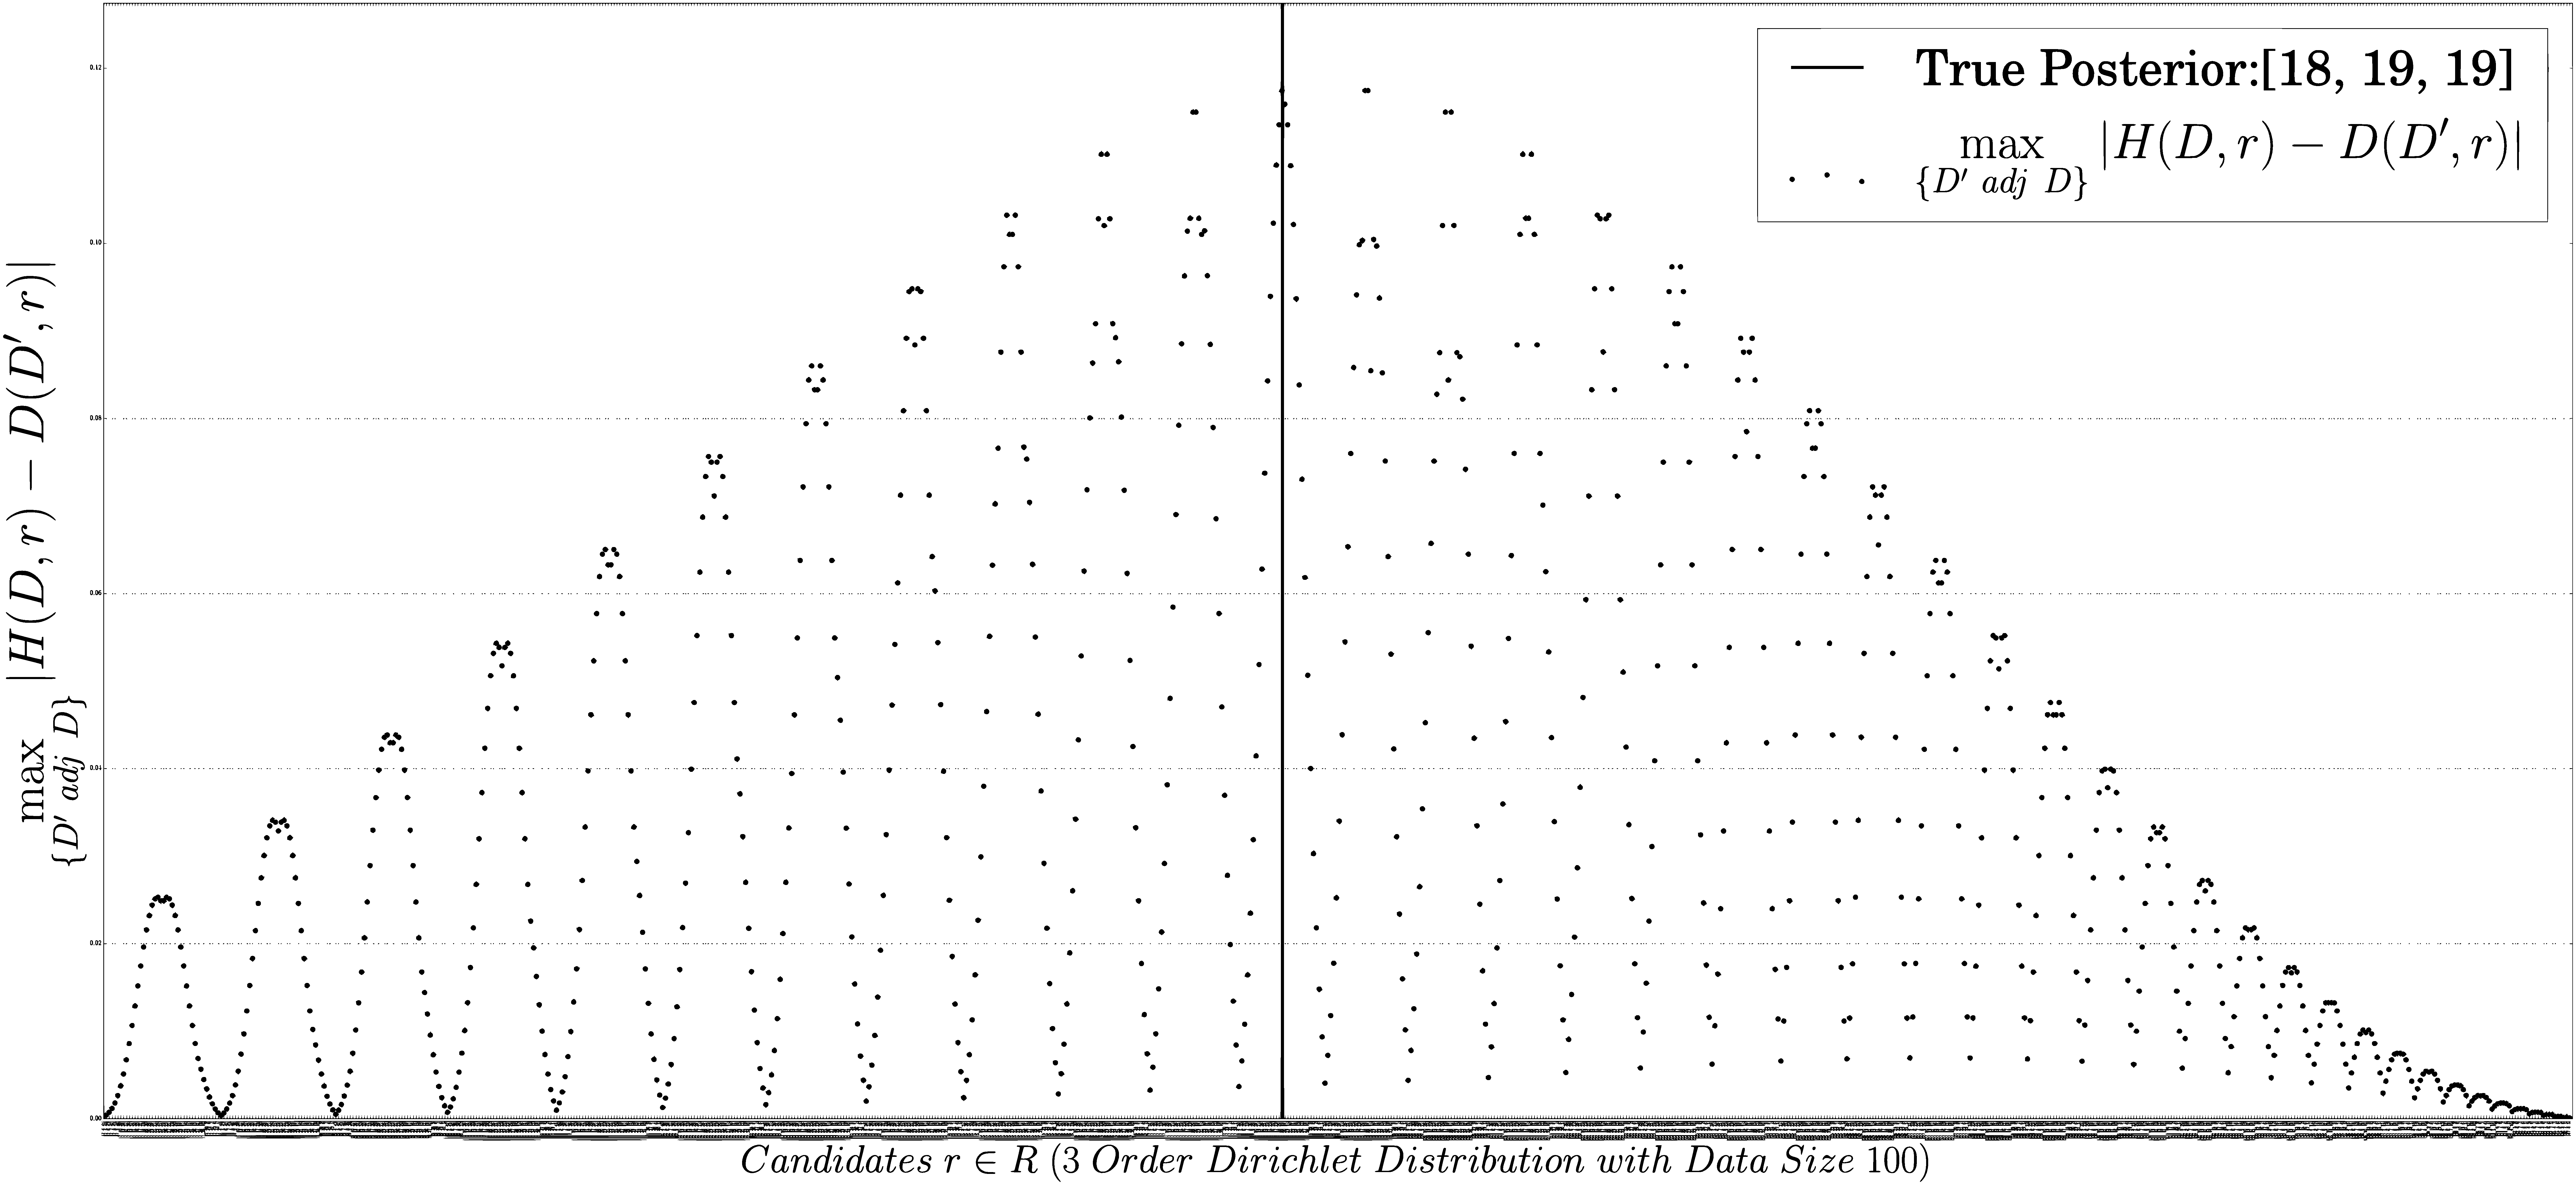
\includegraphics[width=1.0\textwidth]{efficiency}
\label{fig_efficiency}
\caption{Experimental Results for Finding the Local Sensitivity Efficiently}
\end{figure}

\subsection{Accuracy Study Based on Hellinger Distance}
\label{subsec_accuracy_hellinger}
% \begin{figure*}
% \begin{center}
% \centering
%   \subfigure[Data size $n = 300$ with global $\epsilon = 0.5$]{
%     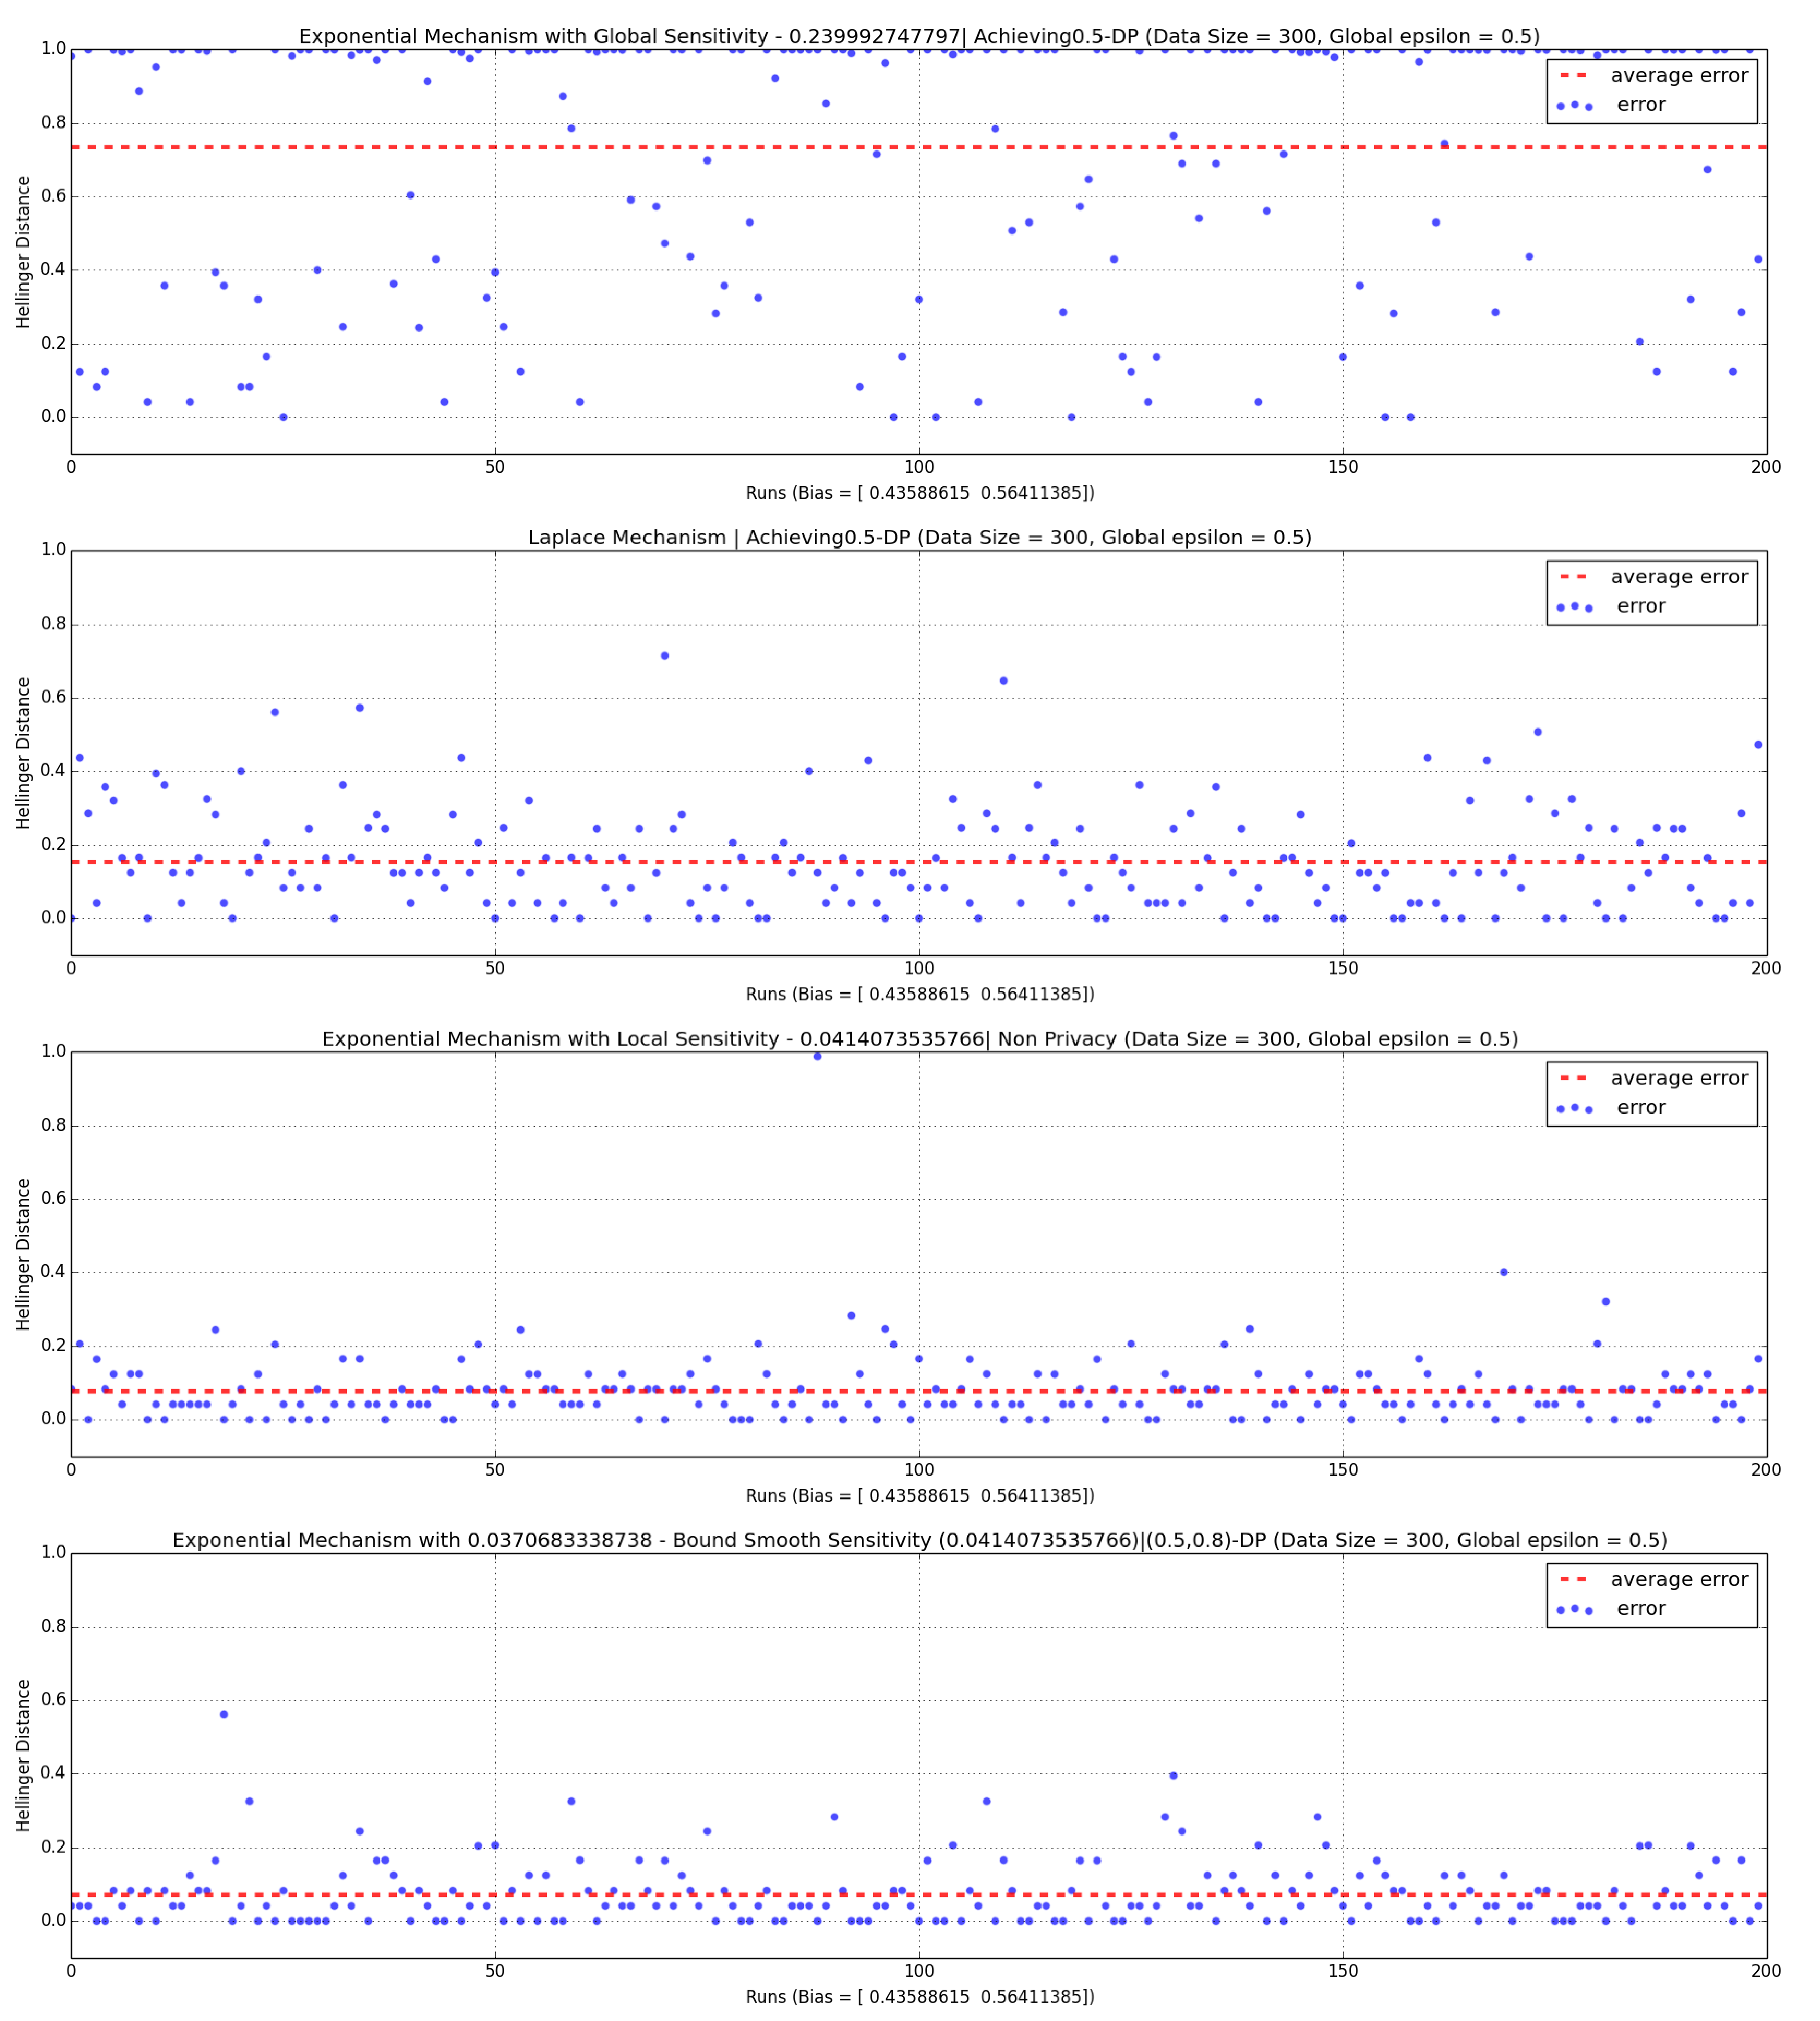
\includegraphics[width=0.48\textwidth]{accuracy_1.eps}}
%   \subfigure[Data size $n = 200$ with global $\epsilon = 0.8$]{
%     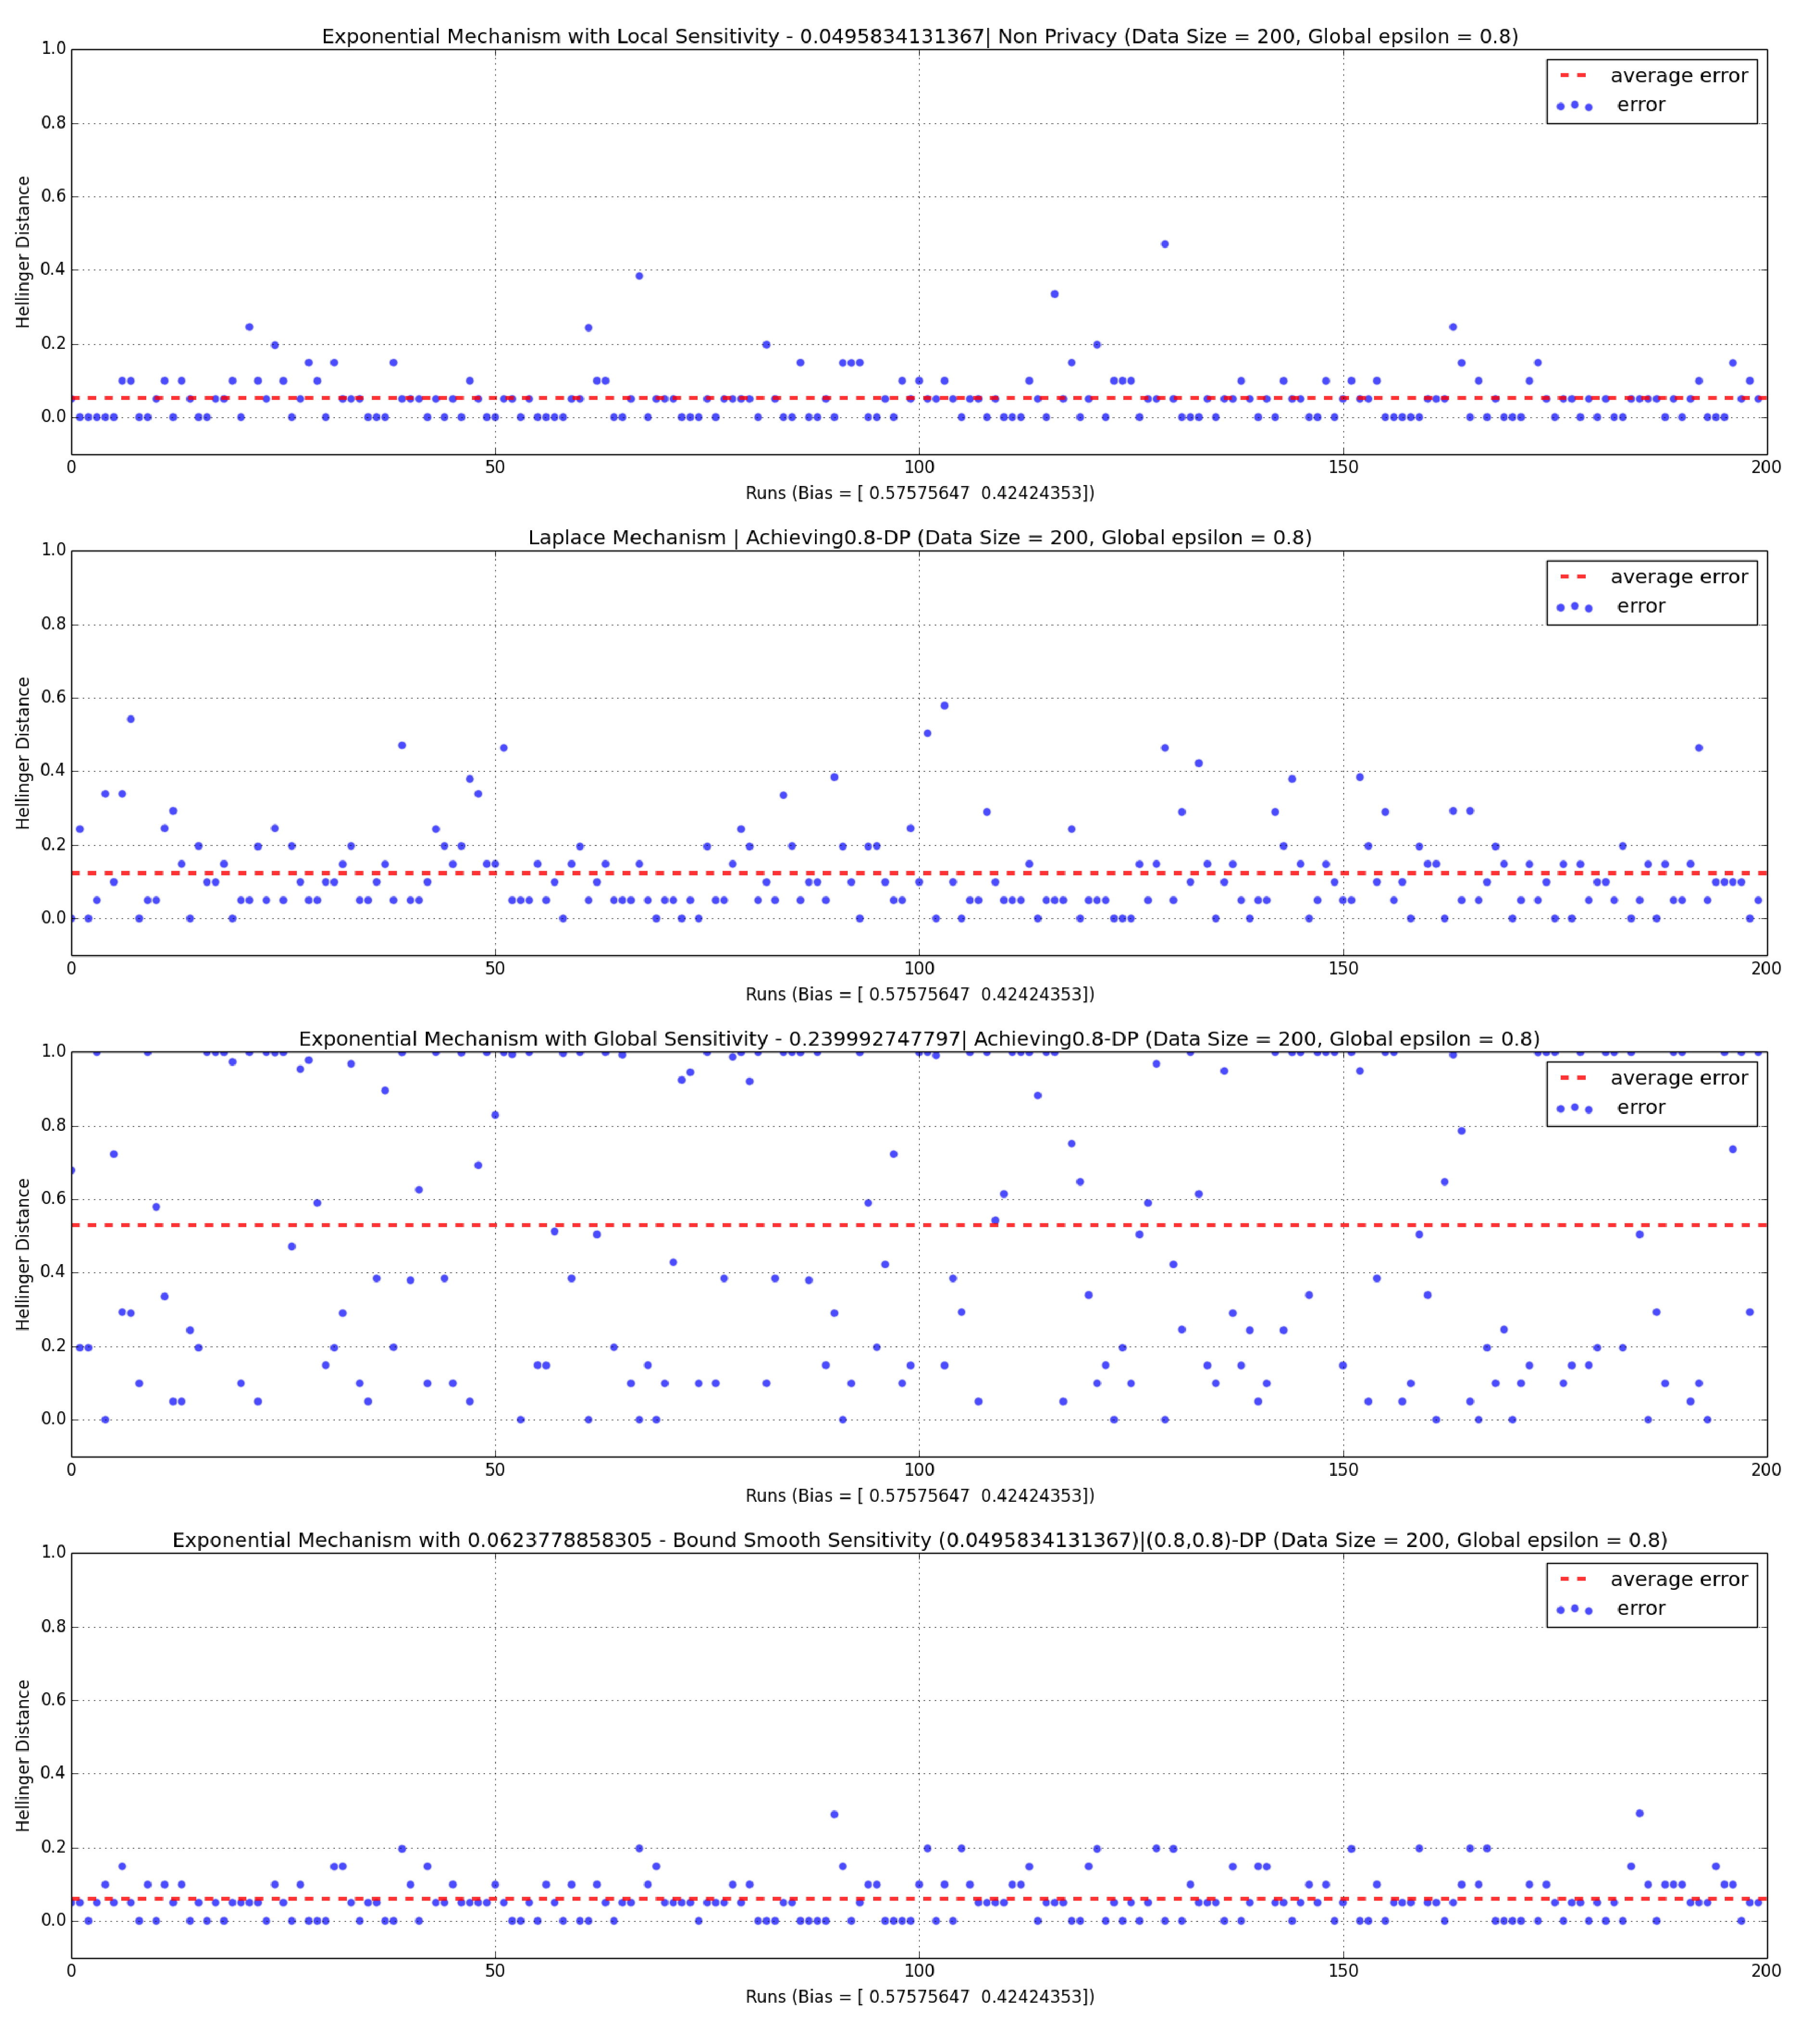
\includegraphics[width=0.48\textwidth]{accuracy_2.eps}} 
% \caption{The experimental results of accuracy of four algorithms}
% \label{fig_data}
% \end{center}
% \end{figure*}
We study the accuracy property of the exponential mechanism with three kind of sensitivity, as well as the Laplace mechanism for comparison. We repeat the experiments for 10000 times and plot their accuracy after every execution. Under different parameters setting, we got two groups of results as in Fig. \ref{fig_beta_hellinger} and Fig. \ref{fig_dirichlet_hellinger}. y-axis is accuracy is measured by Hellinger distance between output $r^*$ and the true inference result $\bysinfer(x)$, $\hlg(r^*, \bysinfer(x))$.


\begin{figure*}
\begin{center}
\centering
  \subfigure[Data size $n = 500$ with global $\epsilon = 0.5$]{
    \includegraphics[width=0.48\textwidth]{accuracy_box_2.eps}}
  \subfigure[Data size $n = 300$ with global $\epsilon = 0.5$]{
    \includegraphics[width=0.48\textwidth]{accuracy_box_1.eps}} 
\caption{The experimental results of accuracy of algorithms with Beta prior distribution $\betad(7,4)$ based on Hellinger distance}
\label{fig_beta_hellinger}
\end{center}
\end{figure*}
When prior distribution is $\betad$, under data size $n = 500$ and $300$, we get two experiment results shown in Fig. \ref{fig_beta_hellinger}.

Then, we extended the $\betad$ to the $\dirichlet$ distribution as well as increase the data size, got the result in Fig. \ref{fig_dirichlet_hellinger}.
\begin{figure*}
\begin{center}
\centering
  \subfigure[Data size $n = 100$, the exponential mechanism with global sensitivity 0.239992747797 is 0.8 -DP, with local sensitivity 0.08 is Non-Private and with 0.0699407108115 - bound smooth sensitivity 0.09 is (0.8,0.8)-DP]{
    \includegraphics[width=0.48\textwidth]{accuracy_dirichlet_hellinger_1.eps}}
  \subfigure[Data size $n = 120$, the exponential mechanism with global sensitivity 0.239992747797 is 0.8 -DP, with local sensitivity 0.0945 is Non-Private, with 0.0677791100173 - bound smooth sensitivity 0.096 is (0.8,0.8)-DP]{
    \includegraphics[width=0.48\textwidth]{accuracy_dirichlet_hellinger_2.eps}} 
\caption{The experimental results of accuracy of algorithms with Dirichlet prior distribution $\dirichlet(7, 4, 5)$ based on Hellinger distance}
\label{fig_dirichlet_hellinger}
\end{center}
\end{figure*}




\subsection{Accuracy Study Based on $L_1$ Norm}
\label{subsec_accuracy_l1}
For comparison, we study the accuracy of these four mechanisms based on $l_1$ norm, with the Dirichlet distribution $\dirichlet(7,4,5)$ and data size $150$, shown in Fig. \ref{fig_dirichlet_hellinger_l1}.

\begin{figure*}
\begin{center}
\centering
  \subfigure[accuracy measurement based on Hellinger distance]{
    \includegraphics[width=0.48\textwidth]{accuracy_compare_dirichlet_hellinger.eps}}
  \subfigure[accuracy measurement based on $l_1$ norm]{
    \includegraphics[width=0.48\textwidth]{accuracy_compare_dirichlet_l1.eps}} 
\caption{The experimental results of accuracy of algorithms with Dirichlet prior distribution $\dirichlet(7, 4, 5)$ based on Hellinger distance and $l_1$  norm, where data size $n = 150$, the exponential mechanism with global sensitivity 0.239992747797 is 0.8 -DP, with local sensitivity 0.0945 is Non-Private, with 0.0677791100173 - bound smooth sensitivity 0.096 is (0.8,0.8)-DP}
\label{fig_dirichlet_hellinger_l1}
\end{center}
\end{figure*}

From results above, we can obtain some preliminary conclusions: 1) Our exponential mechanism with smooth sensitivity can have similar accuracy as it with local sensitivity. Both of the two exponential mechanisms are do much better than it with global sensitivity. 2) The accuracy of our exponential mechanism is better than laplace mechanism. But the advantages are not significant. So we need to have a further exploration on the accuracy trade-off between Laplace mechanism and our exponential mechanism.

\subsection{Accuracy Trade-off Between Laplace and Our Exponential Mechanism with Smooth Sensitivity}
\label{subsec_accuracy_tradeoff}
Based on accuracy study in Sec. \ref{subsec_accuracy_hellinger} and \ref{subsec_accuracy_l1}, we are going to study the relationship between Laplace mechanism and our exponential mechanism further. We will work on some concrete cases based on accuracy bound and probability formula and then have analysis both in theory and experiments.

\subsubsection{Theory Analysis}

\begin{itemize}
	\item In our exponential mechanism, the probability of outputting each candidates are calculated as: which is inversely proportional to the size of candidate size. 
	
	\item
\end{itemize}

\subsubsection{Experiment Analysis}
We studied the accuracy trade-off between our exponential mechanism and Laplace mechanism in experiments. By computing the two mechanisms' discrete probabilities of outputting each candidate separately. Here, we count the probabilities wrt. the steps from correct answer. For example, in the case where the correct posterior distribution is $\betad(5,5)$, the candidate $\betad(4,6)$ and $\betad(6,4)$ are of $1$ steps from $\betad(5,5)$; when correct posterior distribution is $\dirichlet(5,5,5)$, the candidate $\dirichlet(4,5,3)$, $\dirichlet(4,3,5)$, $\dirichlet(5,4,3)$, $\dirichlet(5,3,4)$, $\dirichlet(3,5,4)$ and $\dirichlet(5,5,5)$ are all of $1$ step from $\dirichlet(5,5,5)$. Under the Hellinger distance measurement, if two candidates are of the same steps from correct answer, they also have the same Hellinger distance from correct answer. i.e for every $\hlg(\bysinfer(x), z) = c$, it will have a corresponding steps $step(\hlg(\bysinfer(x), z) = c) = k$.

So in order to be more concise and comparable to the experiment results from Sec. \ref{subsec_accuracy_hellinger}, we sum up the probability values of candidates whose steps (i.e., the hellinger distance) from the correct answer are the same:
\begin{equation*}
\underset{z \thicksim \hexpmech(x)}{Pr}[ \hlg(\bysinfer(x), z) = c] = \sum\limits_{\{z| \hlg(\bysinfer(x), z) = c\}}\frac{exp(\frac{- \epsilon c}{S(x)})}{NL_x}
\end{equation*}

Then we got groups of discrete probabilities wrt. the steps (i.e., Hellinegr distance) from the correct answer, and plotted them. Under different settings, we got same results as in Fig. \ref{fig_theory_50_50}, \ref{fig_theory_20_20_20} and \ref{fig_theory_20_20_20_20}. Subfigs (a) are from Sec. \ref{subsec_accuracy_hellinger} shows the average accuracy of these mechanisms by executing them for 10000 times. x-axis is labeled by each mechanism and y-axis is the accuracy of each executing result measured by Hellinegr distance. We name group (a) as experiment results. Subfigs (b) are concrete probabilities of Laplace and our exponential mechanisms' wrt. the steps. x-axis is the hellinger distance from correct answer, i.e. steps from correct answer. Since they have the same meaning, here we just use the hellinger distance to label the x-axis. The y-axis is the probability of output candidates with corresponding steps from correct answer. We name this group (b) as theory computing results.

\begin{figure*}
\begin{center}
\centering
  \subfigure[accuracy measurement based on Hellinger distance]{
    \includegraphics[width=0.48\textwidth]{theory_compare_50_50.eps}}
  \subfigure[discrete probabilities wrt. hellinger distance]{
    \includegraphics[width=0.48\textwidth]{50_50.eps}} 
\caption{Settings: Dirichlet prior distribution $\dirichlet(1,1)$, observed data $x = (49, 49) $,}
\label{fig_theory_50_50}
\end{center}
\end{figure*}

When the data size is small and the order of the prior distribution is low, our exponential mechanism is better than Laplace, both in experiments and in theory. as shown in Fig. \ref{fig_theory_50_50}.  In Fig. \ref{fig_theory_50_50} (a), the experiment results shown that the average accuracy of our mechanism is better than Laplace mechanism. In the mean time, the theory calculation results in Fig. \ref{fig_theory_50_50} (b) shows our exponential mechanism can output good answer with higher probability and output bad answer with lower probability as well.

\begin{figure*}
\begin{center}
\centering
  \subfigure[accuracy measurement based on Hellinger distance]{
    \includegraphics[width=0.48\textwidth]{theory_compare_20_20_20.eps}}
  \subfigure[discrete probabilities wrt. hellinger distance]{
    \includegraphics[width=0.48\textwidth]{20_20_20.eps}} 
\caption{Settings: Dirichlet prior distribution $\dirichlet(1,1,1)$, observed data $x = (20,20,20) $}
\label{fig_theory_20_20_20}
\end{center}
\end{figure*}

In Fig. \ref{fig_theory_20_20_20}, we plotted these discrete probabilities under the case (x=(20,20,20)). Fig. \ref{fig_theory_20_20_20} (a) shows that the  the This plot shows the laplace mech performs better than ExpMech to some extent but not significant.

\begin{figure*}
\begin{center}
\centering
  \subfigure[accuracy measurement based on Hellinger distance]{
    \includegraphics[width=0.48\textwidth]{theory_compare_20_20_20_20.eps}}
  \subfigure[discrete probabilities wrt. hellinger distance]{
    \includegraphics[width=0.48\textwidth]{20_20_20_20.eps}} 
\caption{Settings: Dirichlet prior distribution $\dirichlet(1,1,1,1)$, observed data $x = (20,20,20,20) $,}
\label{fig_theory_20_20_20_20}
\end{center}
\end{figure*}

In Fig. \ref{fig_theory_20_20_20_20}, we plotted these discrete probabilities under the case ($x=(20,20,20,20)$).  This plot can show clearly that the Laplace Mech are better than Exp Mech when the size is larger and order is higher.  The Laplace can output good answers with much higher probabilities, even though their performances on bad answers are not so obviously.

\begin{figure*}
\begin{center}
\centering
  \subfigure[accuracy measurement based on Hellinger distance]{
    \includegraphics[width=0.48\textwidth]{theory_compare_1_1_1_77.eps}}
  \subfigure[discrete probabilities wrt. hellinger distance]{
    \includegraphics[width=0.48\textwidth]{1_1_1_77.eps}} 
\caption{Settings: Dirichlet prior distribution $\dirichlet(1,1,1,1)$, observed data $x = (1,1,1,77) $,}
\label{fig_theory_1_1_1_77}
\end{center}
\end{figure*}

We also consider an edge case, In Fig. \ref{fig_theory_1_1_1_77}, we plotted these discrete probabilities under the case ($x=(1,1,1,77)$).  This plot can show clearly that the Laplace Mech are better than Exp Mech when the size is larger and order is higher.  The Laplace can output good answers with much higher probabilities, even though their performances on bad answers are not so obviously.

From these cases, we can have conclusions like: 

\bibliographystyle{plain}
\bibliography{bayesian.bib}

\end{document}

